%%%%%%%%%%%%%%%%%%%%%%%%%%%%%%%%%%%%%%%%%%%%%%%%%%%%%%%%%%%%%%%%%%%%%%%%%%%%%%%
%% Template de Relatório Parcial baseado nas normas da ABNT voltado 
%% para alunos da UEFS, baseado no modelo de TCC
%% Versão 1.3
%% Desenvolvimento: Danilo de Oliveira Gonçalves
%% Adaptação final: João Carlos Nunes Bittencourt
%% Data: 31/03/2011
%% Atualização: 11/08/2011
%
% TODO: Ajustar o espaçamento do cabeçalho do Apêndice e do Anexo.
%%%%%%%%%%%%%%%%%%%%%%%%%%%%%%%%%%%%%%%%%%%%%%%%%%%%%%%%%%%%%%%%%%%%%%%%%%%%%%%
\documentclass{abnt-uefs} % Classe de formatação da UEFS
\usepackage[utf8]{inputenc}
%\usepackage[T1]{fontenc}
\usepackage[call=authordata,alf,abnt-emphasize=bf,abnt-etal-text=emph,abnt-and-type=&,abnt-etal-list=3,abnt-etal-cite=3,recuo=0.0cm]{abntex/abntcite}
\usepackage[brazil]{babel}
\usepackage{mathptmx}
\usepackage[pdftex]{graphicx}
%\usepackage[small,bf]{caption}
\usepackage{longtable}
\usepackage{array}
\usepackage{amssymb,amsmath,amsthm,amsfonts}
%\usepackage{textcomp}
%\usepackage{textcase} 
\usepackage{float} % para as figuras ficarem onde foram colocadas no latex - deve colcoar na figura [H]
\usepackage{color}
%\usepackage{url}
\graphicspath{{figuras/}} % Diretório padrão de figuras.
%%%%%%%%%%%%%%%%%%%%%%%%%%%%%%%%%%%%%%%%%%%%%%%%%%%%%%%%%%%%%%%%%%%%%%%%%%%%%%%
% Este arquivo faz parte do template de Relatório Parcial baseado nas normas da ABNT 
%  voltado para alunos da UEFS
% Desenvolvimento: Danilo de Oliveira Gonçalves
% Adaptação final: João Carlos Nunes Bittencourt
% Data: 31/03/2011
% Atualização: 30/11/2011
% Descrição do arquivo:
%   Esse arquivo apresenta as definições de constantes que formarão a capa e 
%   a folha de rosto. Siga as instruções e modifique de acordo com o que
%   lhe foi orientado.
%%%%%%%%%%%%%%%%%%%%%%%%%%%%%%%%%%%%%%%%%%%%%%%%%%%%%%%%%%%%%%%%%%%%%%%%%%%%%%%

% ---------- Preambulo ----------
\instituicao{Universidade Estadual de Maringá} % nome da instituicao
\departamento{Departamento de Informática}
\graduacao{Informática} % nome do curso
\curso{Informática}

\documento{Trabalho de Conclusão de Curso} % tipo de documento
\titulacao{Bacharel} % [Bacharel]

%\titulo{Redes de Computadores} % titulo do trabalho em portugues
\subtitulo{Uso de informações de contexto para controle de acesso em provedores de conteúdo} % caso necessário um sub-título, utilize este campo
%\title{Title in English} % titulo do trabalho em ingles

\autor{Anderson de Souza Zanichelli} % autor do trabalho
\cita{ZANICHELLI, Anderson de Souza Zanichelli} % sobrenome (maiusculas), nome do autor do trabalho

\comentario{\UEFSdocumentodata\ apresentado ao \UEFSdepartamentodata\ como requisito parcial para obtenção do grau de \UEFStitulacaodata\ em \UEFScursodata\ da \ABNTinstituicaodata.}

%\orientador{Profa. Dra. Luciana Andréia Fondazzi Martimiano} % nome do orientador do trabalho
\orientador[Orientadora:]{Profa. Dra. Luciana Andréia Fondazzi Martimiano} % <- no caso de orientadora, usar esta sintaxe
%\coorientador{Nome do Co-orientador} % nome do co-orientador do trabalho, caso exista
%\coorientador[Co-orientadora:]{Nome da Co-orientadora} % <- no caso de co-orientadora, usar esta sintaxe

\local{Maringá} % cidade
\data{2016} % ano



 % Elementos da capa
\begin{document}
    \pagestyle{empty}
    \DeclareGraphicsExtensions{.jpg,.pdf,.mps,.png,.bmp,.eps}
    \capa % geração automática da capa
    \folhaderosto % geração automática da folha de rosto
    %%%%%%%%%%%%%%%%%%%%%%%%%%%%%%%%%%%%%%%%%%%%%%%%%%%%%%%%%%%%%%%%%%%%%%%%%%%%%%%
%% Este arquivo faz parte do template de TCC baseado nas normas da ABNT 
%%  voltado para alunos da UEFS
%% Desenvolvimento: Danilo de Oliveira Gonçalves
%% Adaptação final: João Carlos Nunes Bittencourt
%% Data: 31/03/2011
%%%%%%%%%%%%%%%%%%%%%%%%%%%%%%%%%%%%%%%%%%%%%%%%%%%%%%%%%%%%%%%%%%%%%%%%%%%%%%%


% dedicatória (opcional)
\begin{dedicatoria}
Texto da dedicatória.Texto da dedicatória.Texto da dedicatória.Texto da dedicatória.Texto da dedicatória.Texto da dedicatória.Texto da dedicatória.Texto da dedicatória.Texto da dedicatória.
\end{dedicatoria}

%\vfill

%\begin{flushright}
%\hfill \textit{Dedico esta monografia a minha família,\\pelo apoio fornecido e aos meus amigos.\\}
%\end{flushright}

%\vspace*{1cm}

%\clearpage 

    %%%%%%%%%%%%%%%%%%%%%%%%%%%%%%%%%%%%%%%%%%%%%%%%%%%%%%%%%%%%%%%%%%%%%%%%%%%%%%%
%% Este arquivo faz parte do template de TCC baseado nas normas da ABNT 
%%  voltado para alunos da UEFS
%% Desenvolvimento: Danilo de Oliveira Gonçalves
%% Adaptação final: João Carlos Nunes Bittencourt
%% Data: 31/03/2011
%%%%%%%%%%%%%%%%%%%%%%%%%%%%%%%%%%%%%%%%%%%%%%%%%%%%%%%%%%%%%%%%%%%%%%%%%%%%%%%

% agradecimentos (opcional)
\begin{agradecimentos}
Texto dos agradecimentos.
\end{agradecimentos}

    \begin{resumo}
Com o uso das redes sem fios, que disponibilizam Internet nos dispositivos móveis, a quantidade de serviços e conteúdos oferecidos aos usuários é imensa e como cada provedor de conteúdo que o usuário acessa pode apresentar atributos relacionados aos serviços oferecidos, como por exemplo: número de clientes conectados, tempo de resposta, custo e qualidade do serviço, os valores desses atributos podem ser modificados dependendo da situação do provedor. Dessa forma, o conjunto de atributos pode ser relevante para o usuário no momento da escolha do provedor de conteúdo que atenderá suas expectativas de forma satisfatória, caso não esteja sendo atendido, o usuário irá procurar outro serviço semelhante que lhe atenda da forma desejada. Assim, este trabalho tem como objetivo apresentar esses atributos ao usuário e de forma automatizada escolher e realizar a autenticação no provedor de forma transparente para o usuário.
\end{resumo}	

    \begin{abstract}
With the use of wireless networks that deliver Internet on mobile devices, the number of services and content offered to users is immense and as each content provider that the user accesses may have attributes related to the services offered, such as: number of connected clients, response time, cost and quality of service, the values of these attributes can be modified depending on the provider's situation. Thus, the set of attributes may be relevant to the user when choosing the content provider that will meet your expectations in a satisfactory manner, if not being met, the user will look for another similar service that suits the way the user want. Thus, this study aimed to present these attributes to the user and automated pick and perform authentication on the provider in a transparent manner to the user.
\end{abstract}

    \listadefiguras % geracao automatica da lista de figuras
    \listadetabelas % geracao automatica da lista de tabelas
    \listadesimbolos % geracao automatica da lista de símbolos
    \listadesiglas % % geracao automatica da lista de siglas
    % sumario
    \sumario % geracao automatica do sumario
    %---------- Primeiro Capitulo ----------
\chapter{Introdução}\label{cha:introducao}
\section{Considerações iniciais}
A evolução tecnológica, presente nos dias de hoje, possibilitou o desenvolvimento de dispositivos móveis que não são mais usados somente para a comunicação, mas para a execução de diversas aplicações que oferecem funcionalidades com alta qualidade de serviço, para as quais, há alguns anos atrás seriam necessários diversos equipamentos dedicados, como por exemplo: câmeras de alta resolução para a gravação de áudio e vídeo, computadores para a comunicação através de redes \sigla{Wi-Fi}{Wireless Fidelity} (\textit{Wireless Fidelity}) e aparelhos dedicados para o uso de \sigla{GPS}{Global Positioning System} (\textit{Global Positioning System}).

Com o aumento do poder de processamento dos dispositivos móveis, estes deixaram de ser apenas instrumentos de comunicação para se tornarem também instrumentos de trabalho e entretenimento.
Com o uso das redes sem fios, que disponibilizam o uso da Internet nos dispositivos móveis, a quantidade de serviços e conteúdos oferecidos aos usuários é imensa. Podem ser utilizados serviços como: correio eletrônico, navegação em sites, troca de mensagens instantâneas, download e upload de arquivos, conexão a bancos de dados, o uso de streaming de áudio e vídeo, e tudo o mais que a Internet possa oferecer.

Todos esses serviços e produtos que estão disponíveis na Internet se beneficiam da qualidade das redes de computadores, como por exemplo, uma boa largura de banda e equipamentos de última geração, mas também podem ser prejudicados por alguma deficiência ou problema que aconteça com a rede, como o defeito em algum roteador, o congestionamento na rede ou uma arquitetura mal dimensionada. Assim, cada um dos provedores de conteúdo que o usuário acessa pode apresentar atributos relacionados aos serviços oferecidos, como por exemplo: número de clientes conectados, tempo de resposta, custo da licença para usar o serviço e a qualidade do serviço prestada.

Os valores desses atributos podem ser modificados dependendo do contexto em que se encontra esse provedor. Dessa forma, esse conjunto de atributos pode ser relevante para o usuário no momento da escolha do provedor de conteúdo que atenderá as suas expectativas de forma satisfatória. Como essas informações podem ser alteradas, um serviço escolhido poderá não mais atender ao usuário de forma satisfatória, assim ele poderá procurar outro serviço semelhante que lhe atenda da forma desejada.

Neste trabalho, essas informações serão importantes para a escolha do provedor de conteúdo, elas determinarão qual será o provedor que o usuário escolherá. Assim, este trabalho terá como tarefas a implementação de um serviço para dispositivos móveis que realize consultas a um gerente de autenticação (Broker) e a implementação do Broker, que realizará as autenticações necessárias para o usuário nos provedores de conteúdo, de forma transparente, baseando-se nos atributos que o usuário considera como mais relevantes.

Este trabalho tem como base o trabalho realizado na dissertação de mestrado em Ciência da Computação de \cite{praca12}. Ela descreveu um modelo de autenticação baseado em informações de contexto, denominado HandProv, no qual o usuário efetua handover (troca de conexão de um ponto de acesso para outro sem perda ou interrupção dos serviços) de provedores de serviço de forma transparente.

\begin{citacao}
As autenticações podem ser feitas por meios de mecanismos padrões, como digitação de um login e senha. No entanto, o HandProv propõe um modelo de autenticação automática baseado em informações de contexto obtidas do ambiente por meio das entidades envolvidas e dispostas na rede, tais como informações do usuário, do dispositivo móvel, do provedor de serviço, de aplicações, etc, em que o usuário faz uso de uma aplicação para acessar os serviços de um provedor. \cite{praca12}
\end{citacao}

\section{Motivação}
O grande salto na quantidade de dispositivos móveis utilizados pela população em geral, fez com que aparecessem novas necessidades de software. Alguns desses sistemas têm como objetivo a facilitação de resolução de tarefas do cotidiano do usuário.
A disseminação do uso das redes sem fio, Wi-Fi e 3G, que possibilitam aos usuários estarem conectados à Internet, com uma boa largura de banda, faz com que os usuários passem uma parte considerável de seu tempo utilizando serviços e recursos disponibilizados pela rede.
Devido a essa grande quantidade de serviços disponíveis e muitos deles oferecendo o mesmo tipo de conteúdo o usuário tem a opção de escolher o que atenda-o da melhor maneira.
O problema que esse trabalho se propõe a resolver é o de escolher o serviço que melhor atenda as espectativas parametrizadas realizando as autenticações necessárias de forma transparente ao usuário.

\section{Objetivos e Contribuições}
O objetivo geral deste trabalho é o desenvolvimento de um sistema computacional para dispositivos móveis, tal que se comunique com um servidor (Broker), que realizará autenticações para o usuário, de forma transparente, em provedores de conteúdo, utilizando informações de contexto para a escolha de provedores que atendam os requisitos de qualidade de serviço definidos pelo usuário.
Através dos estudos realizados das tecnologias utilizadas e das implementações dos sistemas, este trabalho ficará disponível à comunidade acadêmica como um exemplo de uma aplicação desenvolvida para dispositivos móveis que utiliza novas tecnologias, como por exemplo um banco de dados NoSQL\footnote{Sistemas de bancos de dados que utilizam formas de armazenar e devolver dados diferente dos que utilizam tabelas relacionais} e o desenvolvimento utilizando ferramentas disponibilizadas na nuvem.

\section{Organização do trabalho}
Neste trabalho o termo 'Dispositivos Móveis' será utilizado para representar o termo em inglês Smartphones, que categoriza uma linha de aparelhos celulares com sistemas operacionais multitarefas.

Este trabalho está organizado da seguinte maneira: O Capítulo \ref{cha:introducao} apresenta o cenário no qual o trabalho se encaixa, a motivação e os objetivos desse trabalho. O Capítulo \ref{cha:fundamentacao} apresenta os principais conceitos sobre autenticação em sistemas computacionais. O Capítulo \ref{cha:visaogeral} apresenta algumas das principais tecnologias sobre dispositivos móveis presentes no mercado atualmente. O Capítulo \ref{cha:ferramentas} apresenta algumas das tecnologias mais conhecidas para o desenvolvimento de aplicativos móveis. O Capítulo \ref{cha:desenvolvimento} apresenta os sistemas que foram implementados e como eles funcionam. O Capítulo \ref{cha:conclusao} finaliza o trabalho de conclusão de curso com as contribuições e trabalhos futuros.

Este documento foi escrito em \LaTeX.
    %---------- Segundo Capitulo ----------
\chapter{Visão geral da área}

As inovações e evoluções em hardware e software dos dispositivos móveis têm atraído atenção de diversos tipos de pessoas, desde usuários leigos que utilizam poucas funcionalidades desses aparelhos aos pesquisadores que utilizam e se beneficiam da mobilidade e da robustez desses novos dispositivos em parte de seus projetos.

\section{Conectividade}
Os dispositivos móveis encontrados no mercado possibilitam que o usuário possam conectá-lo à Internet de alguma forma, sempre utilizando alguma tecnologia de comunicação sem fio, sendo que as mais comuns são as redes locais sem fio \sigla{WLAN}{Wireless Local Area Network} e as redes de telefonia móvel (Celular).
\subsection{WLAN}
Ultimamente o uso da tecnologia de conexão à rede sem fios espalhou-se por todos os lugares, em casa, na universidade, no trabalho, nos aeroportos, hoteis, até em alguns restaurantes.
As redes \textit{Wireless} são conhecidas como redes Wi-Fi, elas abrangem as tecnologias 802.11 do padrão \sigla{IEEE}{Institute of Electrical and Electronics Engineers}.
\begin{citacao}
Wi-Fi é o nome associado à família do padrão IEEE 802.11\footnote{ieee802.org/11/index.shtml}. Assim como o
padrão 802.15, esse padrão opera em faixas de freqüências que não necessitam de licença para instalação e operação. Suas faixas de freqüência são 2,4GHz, 3,6GHz e 5GHz. As aplicações do padrão 802.11 diferem do padrão 802.15 quanto à utilização da rede e a mobilidade do usuário. Wi-Fi oferece alta potência de transmissão e cobre distâncias maiores, oferecendo redes sem fio locais (WLAN). (VANNI, 2009)
\end{citacao}
Uma das maiores vantagens das redes Wi-Fi é a sua compatibilidade com praticamente todos os sistemas operacionais, incluíndo dipositivos como impressoras e video-games.

As redes Wi-Fi fazem o uso das ondas de rádio para transmitir informações e os dispositivos devem ter um adaptador que traduzem os dados em sinais de rádio. Esses sinais são transmitidos através de uma antena para um decodificador conhecido como roteador, que decodifica os sinais e envia os dados para a Internet através de uma conexão com fios à rede \sigla{LAN}{Local Area Network}.

Como as redes Wireless funcionam recebendo e emitindo sinais, os dados recebidos da Internet são codificados em sinais de rádio pelo roteador e recebidos pelo adaptador do dispositivo conectado.
Os pontos de acesso às redes Wi-Fi podem ser públicas, como por exemplo nos aeroportos e restaurantes ou fechadas, como nos locais de trabalho e nas casas.

\begin{figure}[!htb]
	\centering
	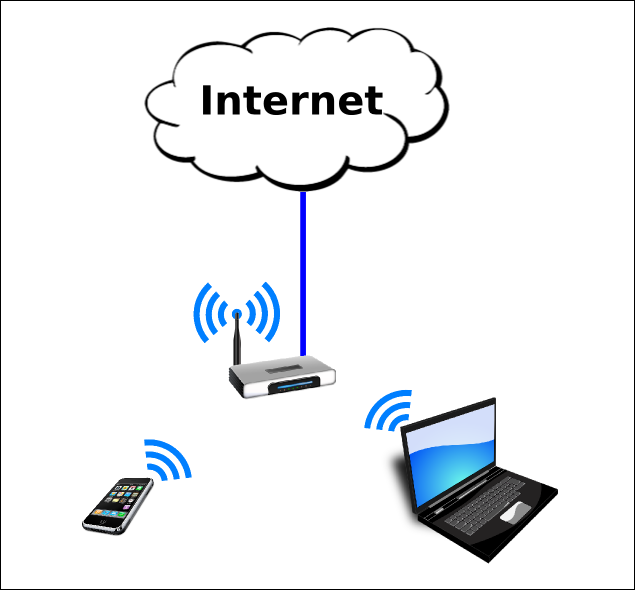
\includegraphics[width=0.6\textwidth]{wlan.png} % <- formatos PNG, JPG e PDF
	\caption[Exemplo da organização de uma WLAN]{Exemplo da organização de uma WLAN.}
	\label{fig:wlan}
\end{figure}

Pelo fato de não ser necessário ter acesso físico aos pontos de acesso, qualquer dispositivo com adaptador wireless poderia ter acesso à Internet através de qualquer roteador Wi-Fi que estivesse no seu alcance. Para bloquear esse acesso às redes Wi-Fi são utilizadas diversas tecnicas de autenticação com protocolos de criptografia como por exemplo:
\begin{itemize}
  \item \sigla{WEP}{Wired Equivalent Privacy}
  - É um algorítmo de segurança que foi introduzido originalmente como parte do protocolo 802.11 que garantiria a confidencialidade dos dados na rede Wi-Fi, mas infelizmente era um algorítmo fácil de quebrar, assim no ano de 2003 a \sigla{Wi-Fi Alliance}{Uma associação da indústria global sem fins lucrativos} \footnote{wi-fi.org/who-we-are} declarou que o WEP havia sido superado pelo WPA.
  \item \sigla{WPA}{Wi-Fi Protected Access}
  - O WPA e o \sigla{WPA2}{Wi-Fi Protected Access II} são dois protocolos de segurança e programas de certificação de segurança desenvolvidos pela \textit{Wi-Fi Alliance} para proteger redes de computadores sem fio. Foram desenvolvidos em resposta às graves deficiências encontradas por pesquisadores no sistema anterior, o WEP.
  \item \sigla{WPS}{Wi-Fi Protected Setup}
  - Criado pela \textit{Wi-Fi Alliance} e introduzido em 2006, o objetivo deste protocolo é permitir que os usuários domésticos
  possam adicionar novos dispositivos na rede Wi-Fi segura sem a necessidade de entender de protocolos de segurança e sem precisar digitar senhas longas nos dispositivos.
\end{itemize}

\subsection{Telefonia móvel}
A primeira geração de telefones celulares foi lançada na década de 80 e utilizavam o sinal analógico. Eram aparelhos grandes, pouco práticos e inconvinientes para serem carregados pelas pessoas.

Na década de 90 eles foram substituídos pela segunda geração. Os dispositivos móveis passaram a utilizar um sinal digital mais confiável que permitiu o uso de mensagens de texto, ou \sigla{SMS}{Short Message Service}. No entanto, a tecnologia ainda não estava robusta ou rápida o suficiente para lidar com os milhares, e depois milhões, de consumidores que queriam usar telefones celulares. Houve também uma demanda crescente para a transmissão de dados através dos celulares.

A tecnologia 2G não era rápida e confiável o suficiente. Então foi desenvolvida uma tecnologia intermediária, chamada de EDGE ou 2.5G, mas foi com a adoção do 3G que se alcançou rapidez e confiabilidade adequadas para o uso da Internet nos dispositivos móveis.
\begin{citacao}
A tecnologia UMTS (Universal Mobile Telecommunications System), mais conhecida como 3G\footnote{O nome de mercado da tecnologia UMTS está associado a 3G para enfatizar uma evolução das gerações de tecnologias de telefonia celular (1G, 2G, 2.5G); é também conhecida como 3GSM para enfatizar sua estreita ligação com a tecnologia GSM}, foi especificada pelo grupo 3GPP\footnote{O projeto 3GPP é uma iniciativa global com o escopo original de desenvolver especificações e relatórios técnicos para sistemas de Terceira Geração que evoluíssem de redes GSM. Atualmente, o projeto inclui também as tecnologias de acesso GSM/GPRS. Página Web do projeto: 3gpp.org/}

UMTS provê serviços de alta transmissão de dados para redes de dados sem fio e telefonia móvel. Essa tecnologia mantém características da segunda geração GSM para telefonia móvel e \sigla{GPRS}{General Packet Radio Service} para redes de dados sem fio. As novas capacidades incluem envio e recebimento de fotos, gráficos e vídeos, além de serviços de voz e dados. (VANNI, 2009)
\end{citacao}

No Brasil estamos vivendo o momento da implantação da tecnologia 4G \sigla{LTE}{Long Term Evolution}, uma evolução do 3G que promete velocidades até 10 vezes mais rápida.

\begin{citacao}
Um dos requisitos do LTE é fornecer taxas de pico downlink de pelo menos 100Mbit/s. A tecnologia permite velocidades acima de 200Mbit/s e a Ericsson já demonstrou taxas acima de 150Mbit/s. Além disso, a latência  deverá ser inferior a 10ms. Efetivamente, isso significa que o LTE – mais do que qualquer outra tecnologia – já atende aos principais requisitos de 4G. (Teleco Inteligência em Telecomunicações\footnote{teleco.com.br/tutoriais/tutoriallte})
\end{citacao}

\begin{table}[!htb]
	\tiny
  	%\centering
	\label{tab:LTE}
	\begin{tabular}{|l|*{8}{c|}}
		\hline \SPACE
		Geração & \multicolumn{3}{|c|}{2G}  & \multicolumn{4}{|c|}{3G}  & 4G\\ \hline \SPACE
		Tecnologia & GSM & GPRS & EDGE & WCDMA & HSPA & HSPA+ & LTE & LTE-Advanced\\ \hline \SPACE
		Downlink & 14,4 Kbps & 171,2 Kbps & 473,6 Kbps & 2,0 Mbps & 7,2/14,4 Mbps & 21/42 Mbps & 100Mbps & 1,0 Gbps\\ \hline \SPACE
		Uplink & - & - & 473,6 Kbps & 474 Kbps & 5,76 Mbps & 7,2/11,5 Mbps & 50 Mbps & 0,5 Gbps\\ \hline \SPACE
		Média teórica & 10-40 kbit/s & 40-50 kbit/s & 100-130 kbit/s & 128-384 kbit/s & 1-10 Mbps & - & - & -\\ \hline \SPACE
		Canalização (MHz) & 0,2 & 0,2 & 0,2 & 5 & 5 & 5 & 20 & 100\\ \hline \SPACE
		Latência (ms) & 500 & 500 & 300 & 250 & ~70 & ~30 & ~10 & <5\\ \hline
	\end{tabular}
	\caption[Evolução da Tecnologia GSM -> LTE-Advanced]{Evolução da Tecnologia GSM -> LTE-Advanced}
\end{table}%\vspace{4cm}
\begin{center}
\small{Fonte: 4gamericas\footnote{4gamericas.org/pt-br/resources/technology-education/3gpp-technology-evolution}}
\end{center}

\section{Sistemas operacionais}
Atualmente existem muitas empresas colocando dispositivos móveis no mercado, cada uma delas opta por um dos sistemas operacionais diponíveis.
Existem sistemas operacionais livres e outros de código fechado, alguns são utilizados apenas em dispositivos da própria fabricante, como no caso do IOS da Apple que é utilizado apenas nos iPhones.

\subsection{Android}
O Android foi desenvolvido pela Google Inc. É um \sigla{SO}{Sistema operacional} construído sobre um kernel Linux e é o SO mais utilizado no mundo nos dispositivos móveis. Ele é de uso geral e além dos dispositivos móveis pode ser utilizado em tablets, TVs, smartwatches e até desktops. Por ser um SO Livre e de Código Aberto muitas empresas o escolhem e o modificam para ser o sistema de seus produtos.
\begin{citacao}
Android é um sistema de software de código aberto criado para uma grande variedade de dispositivos. Os objetivos primordiais do Android são a criação de uma plataforma de software aberto disponível para operadoras, OEMs e desenvolvedores para que tornem as suas ideias inovadoras em realidade e que melhorem as experiências dos usuários. (About Android)\footnote{Tradução livre do texto: source.android.com/source/index.html}
\end{citacao}

\subsection{iOS}
O \sigla{iOS}{iPhone OS} é um sistema derivado do Darwin core OS é o SO utilizado nos dispositivos móveis da Apple Inc., o iPhone. O iOS tem a segunda maior base instalada em dispositivos moveis. É um sistema de código proprietário e de código fechado.
\begin{citacao}
Como a Apple cria tanto o hardware e o sistema operacional para iPad, iPhone e iPod touch, tudo é projetado para trabalhar em conjunto. Assim, os aplicativos tiram o máximo proveito dos recursos de hardware, como o processador dual-core, aceleração gráfica, as antenas wireless, e muito mais. (About iOS)\footnote{Tradução livre do texto: apple.com/ios/what-is/}
\end{citacao}

\subsection{Windows 10 Mobile}
O Windows 10 Mobile é o SO da Microsoft para dispositivos móveis. É o terceiro SO mais utilizado em dispositivos móveis. É de código proprietário e de código fechado.
\begin{citacao}
Windows 10 Mobile é a primeira tentativa da Microsoft para unificar seus sistemas de desktop, tablet e telefone em um único sistema operacional. A versão para dispositivos móveis dispõe de muitos dos mesmos recursos que sua versão para desktop, incluindo o mesmo kernel, elementos da interface, menus e configurações. (Windows Central)\footnote{Tradução livre do texto: windowscentral.com/windows-10-mobile}
\end{citacao}

\begin{table}[!htb]
	%\centering
	\label{tab:OS}
	\begin{tabular}{c|c|c|c|c}
		\hline \SPACE
		\textbf{OS} & \textbf{2015 (Un)}  & \textbf{2015 Market Share(\%)}  & \textbf{2014 (Un)}  & \textbf{2014 Market Share(\%)} \\ \hline \SPACE
		Android & 271.010 & 82,2 & 243.484 & 83,8\\ \hline \SPACE
		iOS & 48.086 & 14,6 & 35.345 & 12,2\\ \hline \SPACE
		Windows Phone & 8.198 & 2,5 & 8.095 & 2,8\\ \hline \SPACE
		BlackBerry & 1.153 & 0,3 & 2.044 & 0,7\\ \hline \SPACE
		Others & 1.229 & 0,4 & 1.416,8 & 0,5\\ \hline \SPACE
		Total & 329.676,4 & 100,0 & 290.384,4 & 100,0\\
		\hline
	\end{tabular}
	\caption[Sistemas operacionais mais utilizados]{Vendas no mundo de Smartphones para usuários finais por sistema operacional em 2015 (Milhares de Unidades)}
\end{table}%\vspace{-1cm}
\begin{center}
	\small
	{Fonte: Gartner, Agosto 2015\footnote{gartner.com/newsroom/id/3115517 Acesso: Dezembro/2015}}
\end{center}
    %---------- Segundo Capitulo ----------
\chapter{Desenvolvimento}
\label{chap:desenv}

A seguir ilustra-se a forma de incluir figuras, tabelas, equa\c{c}\~oes, siglas e s\'imbolos no documento, obtendo indexa\c{c}\~ao autom\'atica em suas respectivas listas. A numera\c{c}\~ao sequencial de figuras, tabelas e equa\c{c}\~oes ocorre de modo autom\'atico. Refer\^encias cruzadas s\~ao obtidas atrav\'es dos comandos {\ttfamily \textbackslash label\{\}} e {\ttfamily \textbackslash ref\{\}}. Por exemplo, n\~ao \'e necess\'ario saber que o n\'umero deste cap\'itulo \'e~\ref{chap:desenv} para colocar o seu n\'umero no texto. Isto facilita muito a inser\c{c}\~ao, remo\c{c}\~ao ou reloca\c{c}\~ao de elementos numerados no texto (fato corriqueiro na escrita e corre\c{c}\~ao de um documento acad\^emico) sem a necessidade de renumer\'a-los todos.

\section{Figuras}

Na figura~\ref{fig:dummy} \'e apresentado um exemplo de gr\'afico flutuante. Esta figura aparece automaticamente na lista de figuras. Para uso avan\c{c}ado de gr\'aficos no \LaTeX, recomenda-se a consulta de literatura especializada~\cite{Goossens2007}.

\begin{figure}[!htb]
	\centering
	\caption[Exemplo de uma figura]{Exemplo de uma figura onde aparece uma imagem sem nenhum significado especial.}
	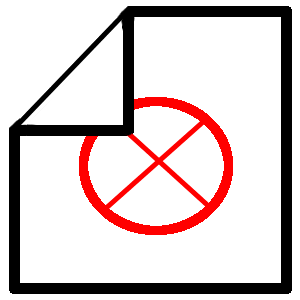
\includegraphics[width=0.2\textwidth]{dummy.png} % <- formatos PNG, JPG e PDF
	\fonte{ABNTEX, 2009\nocite{abnTeX2009}}
	\label{fig:dummy}
\end{figure}

\section{Tabelas}

Tamb\'em \'e apresentado o exemplo da Tabela~\ref{tab:correlacao}, que aparece automaticamente na lista de tabelas. Informa\c{c}\~oes sobre a constru\c{c}\~ao de tabelas no \LaTeX\ podem ser encontradas na literatura especializada~\cite{Lamport1986,Buerger1989,Kopka2003,Mittelbach2004}.

\begin{table}[!htb]
	\centering
	\caption[Exemplo de uma tabela]{Exemplo de uma tabela mostrando a correla\c{c}\~ao entre x e y.}
	\label{tab:correlacao}
	\begin{tabular}{c|c|c|c|c}
		\hline \SPACE
		\textbf{OS} & \textbf{2015 (Un)}  & \textbf{2015 Market Share(\%)}  & \textbf{2014 (Un)}  & \textbf{2014 Market Share(\%)} \\ \hline \SPACE
		Android & 271.010 & 82,2 & 243.484 & 83,8\\ \hline \SPACE
		iOS & 48.086 & 14,6 & 35.345 & 12,2\\ \hline \SPACE
		Windows Phone & 8.198 & 2,5 & 8.095 & 2,8\\ \hline \SPACE
		BlackBerry & 1.153 & 0,3 & 2.044 & 0,7\\ \hline \SPACE
		Others & 1.229 & 0,4 & 1.416,8 & 0,5\\ \hline \SPACE
		Total & 329.676,4 & 100,0 & 290.384,4 & 100,0\\
		\hline 
	\end{tabular}
	\fonte{Pr\'oprio Autor.}
\end{table}

\section{Equa\c{c}\~oes}

A transformada de Laplace \'e dada na equa\c{c}\~ao~(\ref{eq:laplace}), enquanto a equa\c{c}\~ao~(\ref{eq:dft}) apresenta a formula\c{c}\~ao da transformada discreta de Fourier bidimensional\footnote{Deve-se reparar na formata\c{c}\~ao esteticamente perfeita destas equa\c{c}\~oes!}.

\begin{equation}
X(s) = \int\limits_{t = -\infty}^{\infty} x(t) \, \text{e}^{-st} \, dt
\label{eq:laplace}
\end{equation}

\begin{equation}
F(u, v) = \sum_{m = 0}^{M - 1} \sum_{n = 0}^{N - 1} f(m, n) \exp \left[ -j 2 \pi \left( \frac{u m}{M} + \frac{v n}{N} \right) \right]
\label{eq:dft}
\end{equation}

\section{Siglas e s\'imbolos}

O pacote abn\TeX\ permite ainda a defini\c{c}\~ao de siglas e s\'imbolos com indexa\c{c}\~ao autom\'atica atrav\'es dos comandos {\ttfamily \textbackslash sigla\{\}\{\}} e {\ttfamily \textbackslash simbolo\{\}\{\}}. Por exemplo, o significado das siglas\sigla{CCECOMP}{Colegiado do Curso de Engenharia de Computa\c{c}\~ao},\sigla{DAEComp}{Diretório Acad\^emico de Engenharia de Computa\c{c}\~ao} e\sigla{UEFS}{Universidade Estadual de Feira de Santana} aparecem automaticamente na lista de siglas, bem como o significado dos s\'imbolos\simbolo{$\lambda$}{comprimento de onda},\simbolo{$v$}{velocidade} e\simbolo{$f$}{frequ\^encia} aparecem automaticamente na lista de s\'imbolos. Mais detalhes sobre o uso destes e outros comandos do abn\TeX\ s\~ao encontrados na sua documenta\c{c}\~ao espec\'ifica~\cite{abnTeX2009}.

    
\chapter{Fundamentação Teórica}
\label{chap:fundam}

\textcolor{red}{Apresentar estudos que contemple a temática abordada. Respeitar a autoria,
nas citações diretas e indiretas. Evitar parágrafos muito longos. Evitar seções e
subseções muito curtas.}

    
\chapter{Metodologia}
\label{chap:metodo}
\textcolor{red}{Descrever as principais ações realizadas. É preciso justificar, com base na
literatura, a escolha feita pela metodologia, técnicas e instrumentos.}


    \chapter{Resultados}
\label{chap:resul}
Apresentar os resultados da sua pesquisa.
    \chapter{Considerações Finais}
\label{chap:conclusao}
Espera-se que o uso do estilo de formata\c{c}\~ao \LaTeX\ adequado \`as Normas para Elabora\c{c}\~ao de Trabalhos de Conclusão de Curso dos estudantes de Engenharia de Computação, da UEFS ({\ttfamily abnt-uefs.cls}) facilite a escrita de documentos no \^ambito desta institui\c{c}\~ao e aumente a produtividade de seus autores. Para usu\'arios iniciantes em \LaTeX, al\'em da bibliografia especializada j\'a citada, existe ainda uma s\'erie de recursos~\cite{CTAN2009} e fontes de informa\c{c}\~ao~\cite{TeX-Br2009,Wikibooks2009} dispon\'iveis na Internet.

Recomenda-se o editor de textos Kile como ferramenta de composi\c{c}\~ao de documentos em \LaTeX\ para usu\'arios Linux. Para usu\'arios Windows recomenda-se o editor \TeX nicCenter~\cite{TeXnicCenter2009}. O \LaTeX\ normalmente j\'a faz parte da maioria das distribui\c{c}\~oes Linux, mas no sistema operacional Windows \'e necess\'ario instalar o software MiK\TeX~\cite{MiKTeX2009}.

Al\'em disso, recomenda-se o uso de um gerenciador de refer\^encias como o JabRef~\cite{JabRef2009} ou Mendeley~\cite{Mendeley2009} para a cataloga\c{c}\~ao bibliogr\'afica em um arquivo Bib\TeX, de forma a facilitar cita\c{c}\~oes atrav\'es do comando {\ttfamily \textbackslash cite\{\}} e outros comandos correlatos do pacote abn\TeX. A lista de refer\^encias deste documento foi gerada automaticamente pelo software \LaTeX\ + Bib\TeX\ a partir do arquivo {\ttfamily abnt-uefs.bib}, que por sua vez foi composto com o gerenciador de refer\^encias JabRef.

O estilo de formata\c{c}\~ao \LaTeX\ do curso de Engenharia de Computação da UEFS foi elaborados por João Carlos Nunes Bittencourt (joaocarlos@ecomp.uefs.br), e este exemplo de utiliza\c{c}\~ao adaptado de Diogo Rosa Kuiaski (diogo.kuiaski@gmail.com) e Hugo Vieira Neto (hvieir@utfpr.edu.br). Sugest\~oes de melhorias s\~ao bem-vindas.

    % Aqui começa a bibliografia da monografia
    \bibliographystyle{abnt-alf}
    \bibliography{abnt-uefs}
    % Apêndice e Anexos
    \apendice
    %\chapter{Título do Apêndice A}
bla bla bla bla bla bla bla bla bla bla bla bla

bla bla bla bla bla bla bla bla bla bla bla bla

%%%%%%%%%%%%%%%%%%%%%%%%%%%%%%%%%%%%%%%%%%%%%%%%%%%%%%%%%%%%%%%%%%%%%%

\chapter{Título do Apêndice B}
bla bla bla bla bla bla bla bla bla bla bla bla

bla bla bla bla bla bla bla bla bla bla bla bla

    \anexo
    %
\chapter{Título do Anexo A}
\vspace{-3cm}
Anexo A

%%%%%%%%%%%%%%%%%%%%%%%%%%%%%%%%%%%%%%%%%%%%%%%%%%%%%%%%%%%%%%%%%%%%%%

\chapter{Título do Anexo B}
Anexo B

%%%%%%%%%%%%%%%%%%%%%%%%%%%%%%%%%%%%%%%%%%%%%%%%%%%%%%%%%%%%%%%%%%%%%%

\end{document} 